\subsection{Problema 3}

\textit {“El náufrago satisfecho ofrece hamburguesas sencillas (S), dobles (D) y triples (T), las cuales tienen un costo de \$20, \$25 y \$28 respectivamente. La empresa acepta tarjetas de crédito con un cargo de 5\% sobre la compra. Suponiendo que los clientes adquieren N hamburguesas, las cuales pueden ser de diferente tipo, realice un algoritmo para determinar cuánto deben pagar.”}

\textbf{Modelo}

Puesto que se tienen 3 opciones predefinidas, se optó por realizar un \lstinline{enum} con las 3 opciones especificadas.

\begin{center}
\begin{lstlisting}
enum HamType {
  sencilla('Sencilla', 20),
  doble('Doble', 25),
  triple('Triple', 28);

  final String name;
  final double price;
  const HamType(this.name, this.price);
}
\end{lstlisting}
\end{center}

Con este enum, se lo utilizó dentro del modelo, donde se especifica una cantidad para cada tipo de hamburguesa. Adicionalmente se tienen los métodos para calular el total tomando en cuenta el precio base y la cantidad correspondiente.

\begin{center}
\begin{lstlisting}
class HamburgerModel {
  final HamType hamburger;
  int quantity;

  HamburgerModel({required this.hamburger, this.quantity = 0});

  double get total => hamburger.price * quantity;
}
\end{lstlisting}
\end{center}

\textbf{Controlador}

Primero se tiene una lista con el modelo, por lo que se lo transforma mediante:

\begin{center}
\begin{lstlisting}
final List<HamburgerModel> hamburgers = [
  for(var ham in HamType.values)
    HamburgerModel(hamburger: ham)
];
\end{lstlisting}
\end{center}

Luego se definieron métodos para aumentar y disminuir la cantidad de un determinado tipo de hamburguesa. Estos métodos serán utilizados por los widgets \lstinline{Counter} para mostrar en pantalla la cantidad actual de cada hamburguesa.

\begin{center}
\begin{lstlisting}
  void increaseQty(HamburgerModel ham) {
    ham.quantity++;
  }

  void decreaseQty(HamburgerModel ham) {
    if (ham.quantity > 0) {
      ham.quantity--;
    }
  }
\end{lstlisting}
\end{center}

Luego se tienen los métodos para calcular el total a pagar, esto se lo hace recorriendo la lista principal y llamando al método \lstinline{total} para sumar acumulativamente los valores.

\begin{center}
\begin{lstlisting}
double get total {
  double hamTotal = 0;
  for(int i=0; i<hamburgers.length; i++) {
    hamTotal += hamburgers[i].total;
  }
  return hamTotal;
}
\end{lstlisting}
\end{center}

Luego, en caso de que se tenga recargo por la tarjeta de crédito, se obtiene el valor del recargo en base al total de toda la venta. Adicionalmente se tiene con un método que verifica si no se ha seleccionada ninguna hamburguesa, si este es el caso, se devolverá un mensaje de error.

\begin{center}
\begin{lstlisting}
double get charge {
    return total * RECARGO;
  }

String allHamburgersZero() {
  for(int i=0; i<hamburgers.length; i++){
    if(hamburgers[i].quantity != 0) {
      return "";
    }
  }
  return "Agregue por lo menos una hamburguesa";
}
\end{lstlisting}
\end{center}

\textbf{Vistas}

Dentro de la vista, se utiliza el controlador, junto con variables para el manejo del mensaje de error y si se ha aplicado el método de pago por tarjeta de crédito.

\begin{center}
\begin{lstlisting}
final hamCtrl = HamburgerController();
bool _isCreditCardPayment = false;
String _errMsg = "";
\end{lstlisting}
\end{center}

Cuando el usuario presiona el botón para calcular el pago se utiliza el controlador, luego se verifica si se ha seleccionado al menos una hamburguesa, luego se comprueba si hay un recargo si se pagó con tarjeta de crédito, para finalmente pasar a la pantalla de resutlados con los argumentos correspondientes.

\begin{center}
\begin{lstlisting}
void _computeAllHamburgers() {
 setState(() {
   _errMsg = hamCtrl.allHamburgersZero();
 });

  if(_errMsg != "") {
    return;
  }

  double charge = 0;
  if(_isCreditCardPayment){
    charge = hamCtrl.charge;
  }

  Navigator.pushNamed(
    context, "/hamburger/result",
    arguments: {
      'total': hamCtrl.total,
      'recargo': charge,
      'hamburgesas': hamCtrl.hamburgers,
    }
  );
}
\end{lstlisting}
\end{center}

Luego, en la pantalla de resultados, se recuperaron los argumentos mediante:

\begin{center}
\begin{lstlisting}
final args = ModalRoute.of(context)!.settings.arguments as Map<String, dynamic>;

final double total = args['total']!;
final double recargo = args['recargo']!;
final List<HamburgerModel> hamburguesas = args['hamburgesas']!;
\end{lstlisting}
\end{center}

\textbf{Ejecución}

De esta manera se pudo cumplir con el ejercicio propuesto, donde se dan a mostrar 3 opciones de hamburguesa con la posibilidad de poder realizar el pago con tarjeta con una comisión adicional mediante las siguientes pantallas:

\begin{figure}[H]
    \centering
    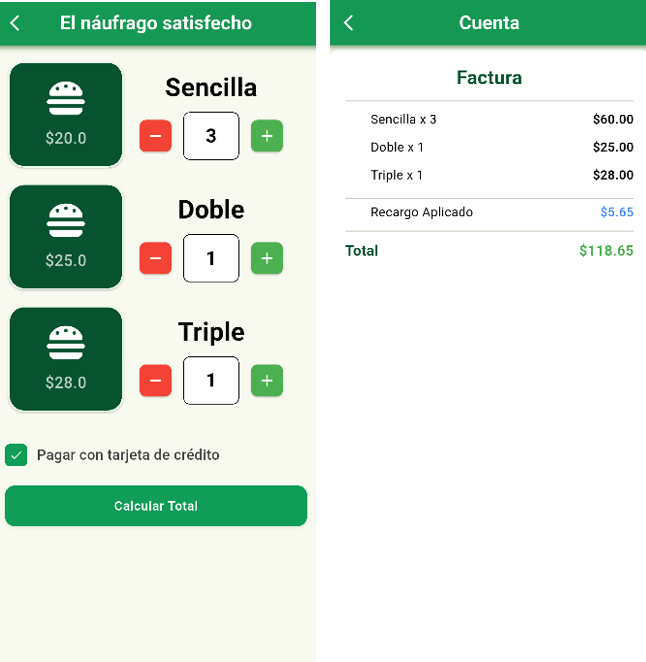
\includegraphics[width=0.8 \textwidth, height=10cm, keepaspectratio]{ejecucion_ej3.png}
    \caption{Ejecucción ejercicio 3}
    \label{fig:ej3_ejecuccion}
\end{figure}